\chapter{Evaluation} \label{chap:eval}

% Proofread: None
The project was highly successful. All success criteria set forth in the project proposal (see \cref{appendix:proposal}) have been met, and many optional extensions implemented, as shown by \cref{table:eval-project-requirements}. The incremental solver achieves sub-second scheduling latency on a 12,000 machine cluster, with a $14.5\times$ speedup over state-of-the-art reference implementations. Approximation yielded a small performance gain on flow scheduling, but significantly underperformed the incremental solver. However, it achieved an over $10\times$ speedup on other classes of flow networks, suggesting it may be profitably employed in other domains.

\begin{table}
    \centering
    % eliminate section prefix
    \crefformats{chapter,section,subsection,appendix,subappendix,subsubappendix}{#2#1#3}
    \crefnames{chapter,section,subsection,appendix,subappendix,subsubappendix}{}{}
    \begin{tabular}{clcccc}
        \textbf{\#} & \textbf{Deliverable} & \textbf{Section}
        \tabularnewline
        \hline
        & \textit{Success criteria} \tabularnewline
        S1 & Implement standard flow algorithms & \cref{sec:impl-cycle-cancelling,sec:impl-ssp,sec:impl-relax,sec:impl-cost-scaling} \tabularnewline
        S2 & Design an approximate solver & \cref{sec:impl-approx} \tabularnewline
        S3 & Integrate system with Firmament & \cref{sec:eval-test-integration} \tabularnewline
        S4 & Develop a benchmark suite & \cref{appendix:impl-benchmark-harness} \tabularnewline
        \hline
        & \textit{Optional extensions} \tabularnewline
        E1 & Design an incremental solver & \cref{sec:impl-incremental} \tabularnewline
        E2 & Build cluster simulator & \cref{sec:impl-firmament} \tabularnewline
        E3 & Optimise algorithm implementations & \cref{sec:eval-optimisations} \tabularnewline
        \hline
    \end{tabular}
    % restore section values
    \crefsections
    \caption[Summary of work completed]{Summary of work completed: deliverables for the project, with the section describing their implementation.}
    \label{table:eval-project-requirements}
\end{table}

\section{Correctness testing}

% For a project of this scope, it is easy for 

% Could link this back to development approaches
% Or just some generic bilge
% Tested individually and when integrated into the system
% Essential for each component to be verified: e.g. standard algorithm implementation being wrong could cause bugs which are hard to track down.

Unit tests were developed for each component. In accordance with the spiral model proposed in \cref{sec:prep-management-model}, these were re-run as a regression test at the end of each development cycle. Integration tests were also performed as soon as the requisite components had been implemented.

\subsection{Unit tests} \label{sec:eval-testing-unit}

Each flow algorithm was tested by comparing the solutions to those produced by a reference implementation. Standard unit test frameworks are not designed to work with the large, external datasets such as flow networks. Consequently, I developed my own test harness in Python to automate verification of flow algorithms. Tests of smaller components, such as data structures, were written using the GTest framework (see \cref{sec:prep-tools-libraries}).

\subsection{Integration tests} \label{sec:eval-test-integration}

In practice, the algorithms developed in this project would be used as part of a larger cluster scheduling system. To demonstrate this capability, the solvers implemented in this project were integrated into the Firmament system. \Cref{fig:firmament-ui} shows the system in action, on a cluster of 14 machines.

\begin{figure}
    \begin{subfigure}{\textwidth}
        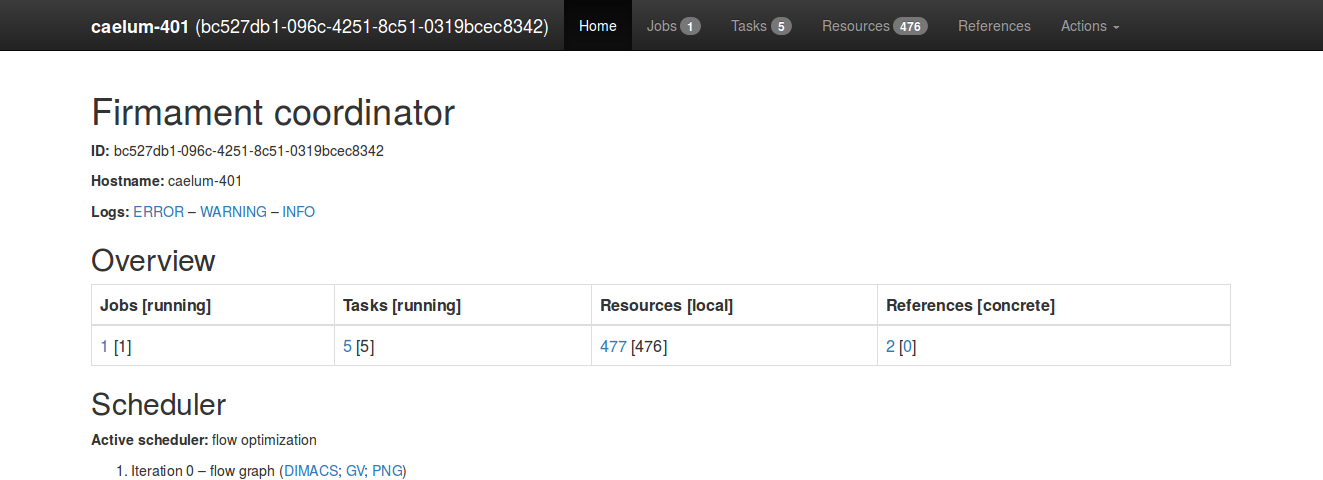
\includegraphics[width=\textwidth]{screenshots/Firmament_overview}
        \caption{An overview from the web user interface for Firmament.}
    \end{subfigure}
    \begin{subfigure}{\textwidth}
        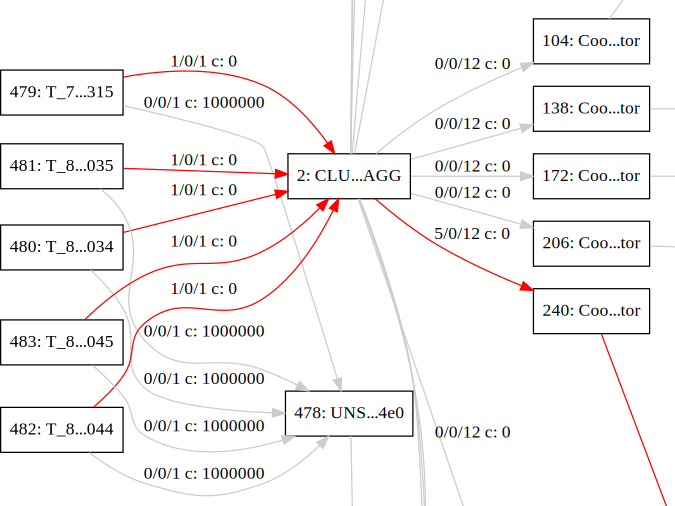
\includegraphics[width=\textwidth]{screenshots/Firmament_flow_graph}
        \caption{An extract of a flow graph, showing the scheduling of a small number of tasks (left hand side). Arcs are \textbf{\color{red} red} if they carry flow, \textbf{\color{gray} grey} otherwise.}
    \end{subfigure}
    \caption[Firmament scheduling tasks]{Firmament scheduling tasks using <TBC:PNAME>}
    \label{fig:firmament-ui}
\end{figure}

\section{Performance testing strategy} \label{sec:eval-benchmark-strategy}

The goal of this project is to improve the performance of flow schedulers: consequently, benchmarking forms the majority of this evaluation. The dataset used in tests is described in \cref{sec:eval-benchmark-strategy-simulation,sec:eval-benchmark-strategy-octopus,sec:eval-benchmark-strategy-quincy}. Finally, \cref{sec:eval-benchmark-strategy-quincy} outlines the methodology used for the experiments.

\subsection{Simulating a Google cluster} \label{sec:eval-benchmark-strategy-simulation}

This project seeks to develop algorithms which will achieve sub-second scheduling latency on warehouse-scale computers, comprising many thousands of compute nodes. Unfortunately, it is not practical to run experiments on such clusters. Performance evaluation must consequently take place using a simulated cluster\footnotemark.
\footnotetext{This is a limitation common to most distributed systems research, not just Part II projects. Even the Quincy system, with all the resources of Microsoft Research behind it, was only ever tested on a small cluster of 243 machines.}

Firmament includes a cluster simulator, which I modified extensively to support this project (see \cref{sec:impl-firmament}). To ensure the test is realistic, the simulator replays a month-long trace of events from a production Google cluster of 12,000 machines~\cite{clusterdata:Wilkes2011,clusterdata:Reiss2011,Reiss:2012}. This is by far the most detailed trace released by any major cluster operator, enabling an accurate simulation.\todo{Do you agree with this? I've not come across any comparable traces, but I don't feel confident I've not missed anything}

However, the trace is not perfect. To protect commercially sensitive information, much of the data was obfuscated by Google before release. Moreover, some data was simply never recorded: for example, the input file size of tasks. 

Although there is sufficient information to reconstruct the topology of the flow network, some cost models require data that is absent from the trace. The next two sections describe the cost models implemented in simulation, and how the limitations of the dataset were overcome.

\subsection{Octopus cost model} \label{sec:eval-benchmark-strategy-octopus}

The Octopus model implements a simple load balancing policy. Tasks and machines are assumed to be homogeneous. The cost of arcs into a machine are proportional to the load on that machine, resulting in tasks being preferentially scheduled on idle machines. 

This policy is too simplistic to be used in production. However, it serves as a useful baseline for comparison. Producing flow networks that are easy to solve compared to more realistic cost models, it provides an upper bound on the real-world scheduling latency that can be achieved.

\subsection{Quincy cost model} \label{sec:eval-benchmark-strategy-quincy}

Flow scheduling was pioneered by the Quincy system, developed at Microsoft Research~\cite{Isard:2009}. To enable a direct comparison between the two systems, I implemented the Quincy cost model in Firmament (see \cref{sec:prep-flow-scheduling,sec:impl-firmament}). Firmament does not currently support preemption, which required a slight modification to the cost model\footnotemark. Otherwise, the model is as described in the original paper.
\footnotetext{I would expect the runtime of all solvers to be larger with preemption enabled, as there would be more arcs in the network. However, I would not anticipate changes in the relative performance of algorithms.}

In contrast to the Octopus model, Quincy has direct real-world applicability: throughput increased by 40\% and data transfer was reduced by a factor of 3.9~\cite{Isard:2009}. The flow networks produced are considerably more complex, being representative of realistic cost models. Moreover, this complexity can be controlled by specifying the length of the preference lists, supporting scalability testing of the algorithms.

Quincy optimises for data locality, scheduling tasks close to where their input data is stored. To achieve this, the cost of arcs from a task to a machine is made proportional to the network bandwidth consumed were the task to be scheduled on that machine. The costs therefore depend upon location of blocks of input data for a task in the distributed filesystem.

Utilising this fine-grained resource information is a major strength of the Quincy system, and flow scheduling in general. However, it poses a challenge for simulation: such detailed information is not present in the trace, and must instead be estimated. 

Upon starting the simulator, a virtual distributed filesystem is built. Each machine is given 6 TB of simulated storage space, in line with typical specifications for machines in contemporary Google clusters~\cite{Fikes:2010}. Files are replicated across three machines, in accordance with industry standards\footnotemark. Each file consists of 64 MB blocks, as in the Google File System~\cite{Ghemawat:2003}.
\footnotetext{In practice, the replication factor varies with the type of data. For example, it would be higher for critical information such as login credentials, and lower for data such as old e-mail attachments.}

A collection of files is generated to saturate the available storage capacity\footnotemark, with file sizes randomly sampled from a distribution. Unfortunately, Google has not released any information on the file size distribution observed inside the cluster. Instead, I have used data from a similarly sized Facebook cluster to estimate a distribution~\cite{Chen:2012}.
\footnotetext{In practice, a cluster would never run at full disk utilisation, however this distinction is unimportant for this test.}

When a task is submitted, an estimate of its input size $S$ is made. A set of input files is then assigned to the task, by randomly sampling from the distributed filesystem until the cumulative size reaches $S$. Google has not released any information on the input size distribution. For consistency, I have used data from the same Facebook cluster to estimate a distribution~\cite{Chen:2012}.

However, it is possible to do better than simply randomly sampling from this distribution. The Google cluster trace contains information about the runtime of individual tasks, and there is a correlation between runtime and input size. Consequently, I have taken the approach of computing the cumulative probability of the runtime for each submitted task, assigning an input size of the same cumulative probability. So, for example, a task of median runtime will be assigned a median input file size.\todo{Does this explanation make sense to you?}

Given the paucity of the trace data, the simulation cannot be expected to exactly reproduce the behaviour of the original Google cluster. However, I believe that the simulation represents a realistic workload, which could plausibly occur in a production cluster today. The exact distributions used, along with justification for the parameters, is provided in \cref{appendix:test-distributions}.

The exact performance of the algorithms will, of course, depend on the architecture and workload of individual clusters. Most metrics used in this chapter therefore measure \emph{relative} performance, which should be robust to such differences. Absolute runtimes are occasionally reported: while indicative of real-world performance, care should be taken not to generalise beyond the experiments conducted.

\subsection{Test methodology} \label{sec:eval-benchmark-strategy-methodology}

Care was taken to minimise experimental error throughout the test process. However, error cannot be completely eliminated: some variation in runtime is inevitable when executing on a time-sharing operating system. Confidence intervals were computed using Student's $t$-distribution to quantify the error, which in most cases is negligible.

Each test was executed multiple times, with the runtimes across test runs aggregated to increase precision. Five iterations were performed by default, with more test runs being performed if the confidence interval was too wide.

Tests typically compared multiple algorithms, operating on the same dataset. Within each test run, algorithms were executed round-robin. This has the desirable property that each algorithm would tend to be equally affected if the performance of the server were to change over time.

However, significant effort was made to minimise variations in performance between runs. Tests took place on machines dedicated to the experiment, ensuring no interference from other workloads. All machines have the same specification (see \cref{appendix:test-machine-spec}), allowing for absolute runtimes to be compared between experiments.

The algorithms were evaluated at multiple scales, ranging from small clusters that might be used within a private company to warehouse-scale computers used to support large cloud applications. \Cref{table:cluster-sizes} summarises the sizes used throughout the rest of the chapter.

\begin{table}
    \centering
    \begin{tabular}{lcc}
        \textbf{Name} & \textbf{Percentage of Google cluster} & \textbf{Number of machines} \tabularnewline
        \hline
        Small & 1\% & 120 \tabularnewline
        Medium & 5\% & 600 \tabularnewline
        Large & 25\% & 3000 \tabularnewline 
        Warehouse-scale & 100\% & 12,000 \tabularnewline
    \end{tabular}
    \caption{Cluster sizes used in benchmarks}
    \label{table:cluster-sizes}
\end{table}

Running the tests manually would be error-prone, as well as extremely time consuming. A test harness was developed in Python to automate the process, described further in \cref{appendix:impl-benchmark-harness}. This ensures the above methodology is followed for all tests.

%* Ensure each algorithm runs at peak performance, before doing comparisons between algorithms. Optimisations, compilers.
%* Say what you're measuring? Perhaps better introduced in each section.

% Specify what properties we're recording? Online vs offline tests?

\section{Optimisations} \label{sec:eval-optimisations}

This project is primarily concerned with algorithmic improvements, however implementation decisions can have a considerable impact on the performance of flow solvers. Comparing an optimised implementation of one algorithm against an unoptimised version of another algorithm could give misleading results. 

Consequently, care has been taken to ensure that all algorithms considered in this project are implemented efficiently. This section evaluates the optimisations applied to each implementation, describes how parameters were set for each algorithm and how a compiler was selected.

%Structure? You probably do want to merge optimisations into a single figure, as Malte suggested. Or at least, a single figure for each algorithm. FIFO is on it's own, but that's about it.
%
%Scaling factor: you'll do this for both your algorithm and Goldie's.
%
%Compilers: everything. But it's boring so you might just want an extract.
%
%So you could have:
%
%* Optimisations: one section for each algorithm, keep it brief.
%* Scaling factor: brief discussion, just for cost scaling.
%* Compilers.
%
%Alternatively:
%
%* Big figure
%* Successive shortest path - ref figure
%* Relax - ref figure
%* Cost scaling - ref figure, and include it's own figure for scaling factor
%* Compilers - everything
%
%Think I favour second approach. You might wanna make this big master figure, though, since it's kinda dependent upon that actually working. Although guess you could break it up, so maybe no dependency... Think it works better if optimisations build on each other. So e.g. small heap + Djikstra with map? Think it wouldn't be too much work to restructure it to do this, the only one where you have interactions is AP. Datasets: only worth having multiple ones when it varies by scale, really.
\subsection{Successive shortest path algorithm}

\begin{figure}
    \centering
    \includegraphics{opt/ap_relative_1col}
    \caption[Optimisations for successive shortest path]{Optimisations for successive shortest path: speedup relative to the naive implementation with standard Djikstra and big heap. The bars represent the mean speedup over 10 replications, with error bars indicating the 95\% confidence interval.}
    \label{fig:opt-ap}
\end{figure}

As explained in \cref{sec:impl-ssp-optimisations}, it is possible to terminate Djikstra's algorithm as soon as it finds a shortest path to a deficit node, without needing to compute shortest paths to all nodes in the graph. This so-called \emph{partial Djikstra} approach yields considerable performance gains. Shown in green on \cref{fig:opt-ap}, it provides a speedup of over $4\times$.

This inspired a related optimisation, \emph{small heap}. Djikstra's algorithm works by maintaining a priority queue of vertices, implemented using a binary heap in this project (see \cref{sec:impl-ssp-optimisations} for justification of this choice). This results in a $\Theta\left(\lg l\right)$ complexity for priority queue operations, where $l$ is the length of the queue.

In the \emph{big heap} implementation, the heap is initialised to contain all vertices in the graph. \emph{Small heap}, by contrast, is initialised containing just the source vertex. Vertices are inserted into the queue as they are encountered during graph traversal.

Initialising a heap with $n$ elements has cost $\Theta(n)$; by contrast, inserting the elements one at a time has a cost of $\Theta(n\lg n)$. Big heap, therefore, will pay less of an initialisation cost --- at least under standard Djikstra, where each vertex is eventually inserted into the queue. However, the number of elements $l$ in the heap will tend to be larger throughout the lifetime of big heap, making each operation more expensive.

When using standard Djikstra, small heap provides a very small (but statistically significant) speedup. However, a substantial performance gain is achieved when using small heap in conjunction with partial Djikstra. This is because with early termination, the typical length $l$ of the queue is much smaller than the number of vertices $n$ in the graph. Shown in gray on \cref{fig:opt-ap}, partial Djikstra with small heap provides a speedup of around $5\times$ over partial Djikstra with big heap, and over $20\times$ compared with the original implementation.

Two versions of small heap were implemented. To support decreasing the key of elements in the priority queue (a common operation in Djikstra's algorithm), it is necessary to maintain a \emph{reverse index} mapping node IDs to elements in the priority queue. In the big heap, this was implemented using an \emph{array} of length $n$. For the small heap, it is possible to reduce memory consumption by using a \emph{hash table}, storing mappings only for nodes $v$ present in the priority queue.

In practice, the algorithm is not memory bound, and runtime is the primary consideration. Both the array and hash table offer $O(1)$ lookup. The array might be expected to be faster: there is no need to compute a hash function, and a result will always be returned after a single memory read (whereas for the hash table, multiple reads may be required in the event of a collision.) However, the hash table may be faster for large heaps: it can be more efficiently cached, since there is less dead space than in the array.

\Cref{fig:opt-ap} clearly show that the array implementation (in gray) outperforms the hash table version (in blue). It may be that the array is never large enough for capacity cache misses to become a problem. Furthermore, hash tables do not necessarily offer a space advantage. The \emph{load factor}, the number of elements divided by the number of buckets, must be kept low to avoid collisions. Consequently, many buckets will be empty, wasting space.

\todo{Should I say which version of the algorithm I ended up using? It seems obvious -- the one which had the best runtime -- but perhaps it's best stated explicitly?}

\subsection{Relaxation algorithm}

\begin{figure}
    \centering
    \begin{subfigure}[c]{0.49\textwidth}
        \includegraphics{opt/relax_arc_cache_quincy_relative_2col}
        \caption{Quincy cost model}
    \end{subfigure}
    \begin{subfigure}[c]{0.49\textwidth}
        \includegraphics{opt/relax_arc_cache_octopus_relative_narrow}
        \caption{Octopus cost model}
    \end{subfigure}
    \caption[Optimisations for relaxation]{Optimisations for relaxation: speedup from maintaining cache of arcs crossing the cut. The bars represent the mean speedup over 30 replications, with error bars indicating the 95\% confidence interval.}
    \label{fig:opt-relax-cache-arcs}
\end{figure}

The relaxation algorithm repeatedly accesses the set of arcs $\left(S,\overline{S}\right)$ crossing the cut. The main relaxation procedure in \cref{algo:relaxation} and \textproc{AugmentFlow} in \cref{algo:relaxation-augment-flow} only consider arcs $(i,j) \in \left(S,\overline{S}\right)$ for which the reduced cost $c_{ij}^{\boldsymbol{\pi}}$ is zero. By contrast, \textproc{UpdatePotentials} in \cref{algo:relaxation-update-potentials} considers only those arcs with positive reduced cost.

In the naive implementation of the algorithm, the entire list of arcs in the graph is searched until an arc satisfying the above conditions is found. It is possible to instead maintain a cache of arcs $\left(S,\overline{S}\right)$ crossing the cut. This imposes an additional cost whenever $S$ is updated, but allows for iteration over the set to proceed more efficiently. At no additional cost, we can partition this cache into two sets: those arcs with zero reduced cost and those with positive reduced cost\footnotemark. This is more efficient, as the algorithm never needs to access the entire set $\left(S,\overline{S}\right)$.
\footnotetext{Note, by the reduced cost optimality conditions, no arcs in the residual network ever have negative reduced cost.}

The effect of this optimisation varies considerably between flow networks, although it yielded a positive speedup in all experiments performed. Under the Quincy cost model, there is only a modest speedup of just over 20\%. By contrast, in the Octopus cost model arc caching yields a more than $40\times$ speedup\footnotemark.
\footnotetext{Results are given only for the small dataset, as the tests timed out on larger network.}

\subsection{Cost scaling}

\subsubsection{Wave vs FIFO}

\begin{figure}
    \centering
    \includegraphics{opt/cs_wave_vs_fifo_relative_2col}
    \caption[Optimisations for cost scaling]{Optimisations for cost scaling: speedup from using a FIFO vertex queue, rather than the wave topological ordering of vertices. The bars represent the mean speedup over 10 replications, with error bars indicating the 95\% confidence interval.}
    \label{fig:opt-cs-wave-vs-fifo}
\end{figure}

Two versions of Goldberg's cost scaling algorithm are described in \cref{sec:impl-cost-scaling-implementations}, \emph{wave} and \emph{FIFO}. The wave implementation has time complexity $O\left(n^3 \lg \left(nC\right)\right)$ compared to a $O\left(n^2m\lg\left(nC\right)\right)$ running time for FIFO. However, for flow scheduling networks the asymptotic time complexities are the same, as $m = O(n)$ by \cref{lemma:network-num-arcs}. 

\Cref{fig:opt-cs-wave-vs-fifo} shows that FIFO considerably outperforms wave on this problem instance, with a speedup of at least $20\times$. I suspect this is because the FIFO queue contains only active vertices (see \cref{algo:cost-scaling-first-active-refine}). By contrast, in wave each iteration involves a pass over every vertex in the graph (see \cref{algo:cost-scaling-wave-refine}), imposing a significant overhead.

Moreover, the larger the size of the network, the larger the speedup enjoyed under FIFO. This suggests that, although wave may have a tighter bound in general, FIFO may have a better asymptotic bound on flow scheduling networks.

% Could also test out first-active approach: when relabel happens, add s to front of Q rather than rear

\subsubsection{Scaling factor}

\begin{figure}
    \begin{widepage}
    \begin{subfigure}[c]{0.5\textwidth}
        \includegraphics{opt/cs_scaling_factor_2col}
        \caption{My implementation}
    \end{subfigure}
    \begin{subfigure}[c]{0.5\textwidth}
        \includegraphics{opt/cs_goldberg_scaling_factor_2col}
        \caption{Goldberg's implementation}
    \end{subfigure}
    \end{widepage}
    \caption[Parameter selection for cost scaling]{Parameter selection for cost scaling: choosing a scaling factor $\alpha$. The bars represent the mean runtime over 5 replications, with error bars indicating the 95\% confidence interval.}
    \label{fig:opt-cs-scaling-factor}
\end{figure}

Cost scaling computes a series of $\epsilon$-optimal solutions, where $\epsilon$ is reduced by a \emph{scaling factor} $\alpha$ between calls to \textproc{Refine}. A value of $\alpha=2$ was proposed in the original paper by Goldberg and Tarjan~\cite{Goldberg:1987}, and is used in \cref{algo:cost-scaling}. However, this choice is not necessarily optimal. Larger values of $\alpha$ will result in fewer calls to \textproc{Refine}, but each call will take longer to execute. The optimal choice for $\alpha$ varies depending on the problem instance~\cite[\S7]{Goldberg:1997}.

\Cref{fig:opt-cs-scaling-factor} shows how the runtime varies by scaling factor. % on the medium size (600 machine) dataset.
The experiment was conducted on both my version of the algorithm, and Goldberg's reference implementation CS2~\cite{CS2:2009}.

My implementation performs best with a small scaling factor, between $2$ and $6$. Runtime is very similar within this range, although $\alpha=3$ offers a small speedup. Performance significantly degrades at $\alpha = 12$ and above.

Goldberg's solver exhibits the opposite behaviour, enjoying considerable performance gains with larger scaling factors. There are diminishing returns after around $\alpha = 12$, with performance starting getting worse from around $\alpha = 24$. Runtimes are statistically indistinguishable in the range $\alpha=16$ to $24$.

I believe this behaviour is due to Goldberg's extensive use of heuristics (see \cref{appendix:impl-csheuristics}) in his implementation. Although these improve the overall performance of the algorithm, they add overhead to to each execution of \textproc{Refine}. This favours larger values of $\alpha$, which cause fewer calls to \textproc{Refine}. 

In subsequent tests, a scaling factor of $\alpha = 3$ is used for my implementation and $\alpha = 20$ for Goldberg's. These offer small, but statistically significant speedups, over the default cost scaling factors of $2$ (my implementation) and $12$ (Goldberg's implementation).

\subsection{Compilers} \label{sec:eval-optimisations-compilers}

\begin{figure}
    \includegraphics{com/cs_with_legend_compiler_1col}
    \caption[Choosing a compiler for cost scaling]{Choosing a compiler for cost scaling: runtime on GCC and Clang at varying optimisation levels. Experiment conducted on medium (600 machine) cluster. The bars represent the mean runtime over 5 replications, with error bars indicating the 95\% confidence interval.}
    \label{fig:compiler-settings}
\end{figure}

\begin{table}
    \centering
    \begin{tabular}{cp{0.9\textwidth}}
        \textbf{Level} & \textbf{Description}\tabularnewline
        \hline
        O0 & No optimisation. \tabularnewline
        O1 & Optimise to reduce code size and execution time. Do not perform optimisations which could greatly increase compilation time. \tabularnewline
        O2 & Perform optimisations which do not involve a space-speed tradeoff. \tabularnewline 
        O3 & Optimise even more, possibly at the expense of increased binary size. \tabularnewline
    \end{tabular}
    \caption{Optimisation levels supported by GCC and Clang}
    \label{table:optimisation-flags}
\end{table}

\emph{Optimising compilers} apply transformations which preserve the semantic meaning of the program, while (typically) improving performance. Two compilers were evaluated for this project: the GNU C Compiler (GCC) and Clang. Both are well-established, and have extensive optimisation support. In general, neither is better than the other: some programs run faster when compiled with Clang, others with GCC.

In addition to choosing a compiler, it is necessary to decide upon which optimisation level to use: the choices for GCC and Clang are summarised in \cref{table:optimisation-flags}. Higher levels tend to produce faster code, at the cost of longer compilation times. For this project, runtime performance is the overriding concern. However, optimisation is a heuristic process: some aggressive optimisations can actually harm program performance. For example, inlining functions will increase the size of functions, increasing the risk of instruction cache misses. Consequently, the highest level is not necessarily best.

\Cref{fig:compiler-settings} shows the runtime of my cost scaling implementation compiled with GCC and Clang, under all supported optimisation levels. There is a dramatic improvement from applying the lowest level of optimisations, O1. GCC's O1 setting is fairly aggressive, achieving performance comparable to O2. Clang's is more relaxed, but their performance at O2 and O3 are both comparable.

This test was repeated for all other implementations in the project, the results of which are given in \cref{appendix:test-compilers}. Other implementations showed a similar pattern\footnotemark. GCC O3 was always competitive, and sometimes had a slight performance edge over Clang O3, and so is used in all subsequent tests.
\footnotetext{Implementations varied considerably in how much benefit they derived from optimisation, higher optimisation levels never decreased performance. Frangioni's relaxation implementation saw no benefit from an optimising compiler, likely due to it having been extensively hand optimised.}

\section{Approximation algorithm} \label{sec:eval-approx}

Unlike with other algorithms, evaluation of approximate solution methods (see \cref{sec:impl-approx}) must consider not just their speed, but also their accuracy\footnotemark. To complicate matters further, both the speed and accuracy of the approximation algorithm will vary depending on the terminating condition chosen.
\footnotetext{Defined to be the ratio of the cost of an optimal solution, to the cost of the solution returned.}

I introduce an \emph{oracle} policy to ease interpretation of the results. It is assumed that the oracle knows precisely what the cost of the optimal solution is, and will terminate the algorithm as soon as an intermediate solution is found that reaches he target accuracy. Of course, an oracle model could not actually be implemented: the entire challenge of approximation is that the minimum cost is not known \textit{a priori}. The oracle policy therefore provides an upper bound on the speedup that can be achieved by approximation.

To evaluate the heuristic policies (see \cref{sec:impl-approx-adaptions}), I split the dataset into training and test data in a 1:3 ratio. The parameters are chosen from the training data in order to achieve a target accuracy $A$ at least a proportion $p$ of the time. In the tests below, both $A$ and $p$ were set to 99\%. Naturally, relaxing these constraints will allow for a greater speedup.

The accuracy and speed of the algorithm are evaluated by running it on the (unseen) test data, with the parameters chosen in the previous step. This split of test and training data guards against overfitting.

All tests were conducted using my implementation of cost scaling, described in \cref{sec:impl-cost-scaling}. Since the experiments in this section measure runtime \emph{relative} to the same algorithm used as an optimal solver, I believe the results should generalise to other implementations of cost scaling. 

There is one notable exception to this. The oracle policy achieves a speedup even at 100\% accuracy in these experiments, since optimality is often reached when $\epsilon > 1/n$. The \emph{price refinement} heuristic (see \cref{appendix:impl-csheuristics}), present in highly optimised implementations such as Goldberg's CS2~\cite{CS2:2009}, is able to detect such early optimality. Consequently, such implementations would achieve the same performance as the oracle model at 100\% accuracy. Further work is required to determine if any other differences exist.

\todo{This section might be improved by including some example figures. But I want to split up the results into subsections for flow scheduling and other applications, and I'd like to avoid duplicating graphs.}

\subsection{Performance on flow scheduling}

Evaluation took place on flow networks produced by the cluster simulator under the Quincy cost model (see \cref{sec:eval-benchmark-strategy}). A total of 1000 different networks were produced, by varying the seed used to initialise the random number generator. This had the effect of changing the generated simulated filesystem, and the input files associated with each task, with consequent changes to costs and preference arcs.

The flow networks produced by the above method are snapshots of the cluster at the beginning of the trace. An alternative would be to take snapshots from multiple points in time, evaluating the algorithm on the time series. However, many tasks in the Google trace run for the entire month data was collected. Consequently, there is significant correlation between flow networks in the time series, even if days apart.

As a result, the training and test data by the time series method is more similar than would be the case in practice, which would biasing the test in favour of the approximation algorithm. Networks produced by varying the seed, by contrast, are considerably more dissimilar providing a more challenging dataset.

\begin{figure}
    \centering
    \includegraphics{app/quincy_medium_oracle_policy_1col}
    \caption[Upper bound on speedup from approximation with flow scheduling]{Upper bound on speedup from approximation on flow scheduling networks, computed using the oracle policy. The experiment was conducted over 1,000 independently generated networks.}
    \label{fig:app-quincy-medium-oracle}
\end{figure}

\Cref{fig:app-quincy-medium-oracle} shows the maximum speedup that can be achieved by approximation, using the oracle policy. At the 99\% target accuracy, this gives an upper bound of just over 135\%. The confidence intervals are tight, never exceeding 2\%, showing remarkable consistency across the dataset.

Two heuristics, \emph{cost convergence} and \emph{task assignment convergence} were implemented (see \cref{sec:impl-approx-adaptions}). The subsequent sections evaluate how close these heuristic policies come to achieving the bound set by the oracle policy.

\subsubsection{Cost convergence}

\begin{figure}
    \centering
    \includegraphics{app/quincy_medium_policy_cost_parameters_1col}
    \caption[Parameter choice for cost convergence with flow scheduling]{Parameter choice for cost convergence on flow scheduling networks: selecting a cost threshold $c$. Cost convergence was applied, for various parameters $c$, to each of the 250 networks in the training set. The solution accuracy measures how close the resulting solutions were to optimality. $c$ was selected to be $0.01\%$, where the \textbf{\color{matplotlib_blue} 1st percentile} cuts the 99\% target accuracy line.}
    \label{fig:app-quincy-medium-cost-parameters}
\end{figure}

Under cost convergence, the algorithm terminates when the cost changes by less than a factor $c$. \Cref{fig:app-quincy-medium-cost-parameters} shows the accuracy achieved at various percentiles for different parameters. The \textbf{\color{matplotlib_blue} 1st percentile} line, representing the accuracy which is met or exceeded 99\% of the time in the training set, drops precipitously at the left of the graph. Consequently, $c$ is set to a very low value of $0.01\%$. This is not encouraging: such a low threshold will tend to give a correspondingly low speedup.

\begin{figure}
    \begin{widepage}
        \begin{subfigure}[c]{0.5\textwidth}
            \includegraphics{app/quincy_medium_policy_cost_accuracy_narrow_2col}
            \caption{Accuracy CDF}
            \label{fig:app-quincy-medium-cost-cdf:accuracy}
        \end{subfigure}
        \begin{subfigure}[c]{0.5\textwidth}
            \includegraphics{app/quincy_medium_policy_cost_speed_2col}
            \caption{Speedup CDF}
            \label{fig:app-quincy-medium-cost-cdf:speedup}
        \end{subfigure}
    \end{widepage}
    \caption[Performance of cost convergence on flow scheduling networks]{Performance of cost convergence policy on flow scheduling networks. Results computed over the 750 networks in the test set.}
    \label{fig:app-quincy-medium-cost-cdf}
\end{figure}

\Cref{fig:app-quincy-medium-cost-cdf} shows the performance of this policy. 100\% accuracy is achieved in 749 out of 750 cases in the test set. The remaining case, however, has a disappointing 25\% accuracy (off the axis of the graph). There is a significant speedup in all cases, although performance is noticeably behind that of the oracle model. This is unsurprising: since optimality is reached in most cases, the algorithm has performed more work than was necessary.

\subsubsection{Task migration convergence}

\begin{figure}
    \centering
    \includegraphics{app/quincy_medium_policy_task_assignments_parameters_1col}
    \caption[Parameter choice for task migration convergence with flow scheduling]{Parameter choice for task migration convergence on flow scheduling networks: selecting a task migration threshold $t$. As with \cref{fig:app-quincy-medium-cost-parameters}, the policy was applied to the 250 networks in the training set. A threshold $t=6206$ is chosen, where the \textbf{\color{matplotlib_blue} 1st percentile} cuts the 99\% target accuracy line.}
    \label{fig:app-quincy-medium-task-assignment-parameters}
\end{figure}

The task migration convergence heuristic measures the number of tasks that have been reassigned (`migrated') between machines, terminating when it is less than a threshold $t$. Although it was hoped that this domain-specific heuristic might fare better than the more general cost convergence policy, \cref{fig:app-quincy-medium-task-assignment-parameters} is not encouraging. 

% TODO: Graph actually showing task migrations?
Although the number of task migrations falls somewhat as the algorithm converges, it remains high throughout execution. In fact, tasks are migrated even once optimality is reached (but while $\epsilon > 1$)! Tasks with only a single input file will have preference arcs with zero cost to each machine that has a replica of the file; these tasks may be migrated freely between machines in their preference set, without changing the cost of the overall solution.

This is reflected in the fact that accuracy in \cref{fig:app-quincy-medium-task-assignment-parameters} only drops at a relatively large migration threshold, of over $6000$. When it does fall, it does so precipitously, indicating the heuristic will be highly sensitive to parameter setting.

\begin{figure}
    \begin{widepage}
        \begin{subfigure}[c]{0.5\textwidth}
            \includegraphics{app/quincy_medium_policy_task_assignments_accuracy_narrow_2col}
            \caption{Accuracy CDF}
            \label{fig:app-quincy-medium-task-assignment-cdf:accuracy}
        \end{subfigure}
        \begin{subfigure}[c]{0.5\textwidth}
            \includegraphics{app/quincy_medium_policy_task_assignments_speed_2col}
            \caption{Speedup CDF}
            \label{fig:app-quincy-medium-task-assignment-cdf:speedup}
        \end{subfigure}
    \end{widepage}
    \caption[Performance of task migration policy on flow scheduling networks]{Performance of task migration policy on flow scheduling networks. Results computed over the 250 networks in the test set.}
    \label{fig:app-quincy-medium-task-assignment-cdf}
\end{figure}

The performance shown in \cref{fig:app-quincy-medium-task-assignment-parameters} is equally disappointing. The accuracy CDF \cref{fig:app-quincy-medium-task-assignment-cdf:accuracy} exhibits a similar pattern to cost convergence in \cref{fig:app-quincy-medium-cost-cdf:accuracy}. The speedup CDF in \cref{fig:app-quincy-medium-task-assignment-cdf:speedup} is still worse. In the vast majority of cases, \emph{no} speedup occurred: the algorithm does not terminate even once optimality is reached, since tasks continue to be migrated. There are a handful of cases which enjoyed a considerable speedup. These correspond to the 1.6\% of cases which failed to meet the 99\% accuracy target, however, and so can hardly be counted a success.

\subsubsection{Conclusion}

Approximation algorithms do not appear to be a viable means for improving the performance of flow schedulers. The heuristics implemented in this project perform poorly under the Quincy cost model. It is possible that more sophisticated heuristics might improve upon this. However, the oracle policy gives a 135\% upper bound on the speedup. Since order of magnitude performance gains are required to make flow scheduling a reality, approximation is not promising for this application.

\subsection{Performance in other applications}

The method of approximation I developed in this project can be applied to any flow network. Although its performance was disappointing in its intended application, on flow scheduling networks produced by Firmament, it provides a considerable performance gain on other types of network. I employ two network generators, NETGEN~\cite{Klingman:1974} and GOTO~\cite{GoldbergDIMACS:1993}. These have a long history of use in computational benchmarks, having been employed in the first DIMACS Implementation Challenge~\cite{DIMACSChallenge:Book}.

\begin{table}
    \centering
     % Increase space between columns slightly. N.B. Only applies to this table.
    \setlength{\tabcolsep}{1.5em}
    \begin{tabular}{p{0.25\textwidth}p{0.75\textwidth}}
        \textbf{Dataset} & \textbf{Description} \tabularnewline
        NETGEN-8 & Sparse networks, with an average outdegree of $8$. Arc capacities and costs are selected uniformly at random from $\left[1,1000\right]$ and $\left[1,10000\right]$ respectively. Number of supply and demand nodes is set to $\sqrt{n}$, with an average supply of 1000 per node. \tabularnewline
        NETGEN-SR & Dense networks, with an average outdegree of $\sqrt{n}$. Other parameters are the same as NETGEN-8. \tabularnewline
        NETGEN-LO-8 and NETGEN-LO-SR & Like NETGEN-8 and NETGEN-LO-SR, except the average supply per node is 10 instead of 1000. The arc capacities therefore provide only ``loose'' bounds for the feasible solutions. \tabularnewline
        GOTO-8 & Sparse networks, with an average outdegree of $8$. Maximum arc capacity is 1000, maximum arc cost is 10,000. \tabularnewline
        GOTO-SR & Dense networks, with an average outdegree of $\sqrt{n}$. Other parameters are the same as GOTO-8. \tabularnewline
    \end{tabular}
    \caption{Datasets used for benchmarking the approximation algorithm}
    \label{table:general-datasets}
\end{table}

Each generator takes input parameters controlling the structure of the generated network. I use the same set of parameters used in the benchmark from Kiraly and Kovacs~\cite{KiralyKovacs:2012}, summarised in \cref{table:general-datasets}. A 1000 networks were generated of each instance by varying the random seed, with 250 of these networks used for training and the remaining 750 for test data.

\begin{figure}
    \begin{widepage}
    \begin{subfigure}[c]{0.5\textwidth}
        \includegraphics{app/netgen_8_oracle_policy_2col.pdf}
        \caption{NETGEN-8}
    \end{subfigure}
    \begin{subfigure}[c]{0.5\textwidth}
        \includegraphics{app/netgen_lo_8_oracle_policy_2col.pdf}
        \caption{NETGEN-LO-8}
    \end{subfigure}
    \begin{subfigure}[c]{0.5\textwidth}
        \includegraphics{app/netgen_sr_oracle_policy_2col.pdf}
        \caption{NETGEN-SR}
    \end{subfigure}
    \begin{subfigure}[c]{0.5\textwidth}
        \includegraphics{app/netgen_lo_sr_oracle_policy_2col.pdf}
        \caption{NETGEN-LO-SR}
    \end{subfigure}
    \begin{subfigure}[c]{0.5\textwidth}
        \includegraphics{app/goto_8_oracle_policy_2col.pdf}
        \caption{GOTO-8}
    \end{subfigure}
    \begin{subfigure}[c]{0.5\textwidth}
        \includegraphics{app/goto_sr_oracle_policy_2col.pdf}
        \caption{GOTO-SR}
    \end{subfigure}
    \end{widepage}
    \caption[Upper bound on speedup from approximation on general flow networks]{Upper bound on speedup from approximation on general flow networks, computed using the oracle policy. The experiment was conducted over 1,000 independently generated networks.}
    \label{fig:app-general-oracle-policy}
\end{figure}

\Cref{fig:app-general-oracle-policy} shows the maximum speedup that can be achieved on each class of networks. Note that a considerably greater speedup is possible on networks produced by NETGEN, in the first two rows, than those of GOTO, on the last row. This highlights that performance is highly dependent on the class of flow networks. The tightly constrained networks, in the top row, enjoy more of a speedup than the loosely constrained ones, in the second row. The speedup on the dense network NETGEN-SR is greater than for the sparse network NETGEN-8, however this pattern is reversed for GOTO-SR and GOTO-8.

\begin{figure}
    \begin{widepage}
        \begin{subfigure}[c]{0.5\textwidth}
            \includegraphics{app/netgen_8_policy_cost_parameters_2col.pdf}
            \caption{NETGEN-8}
        \end{subfigure}
        \begin{subfigure}[c]{0.5\textwidth}
            \includegraphics{app/netgen_lo_8_policy_cost_parameters_2col.pdf}
            \caption{NETGEN-LO-8}
            \label{fig:app-general-cost-parameters:netgen-lo-8}
        \end{subfigure}
        \begin{subfigure}[c]{0.5\textwidth}
            \includegraphics{app/netgen_sr_policy_cost_parameters_2col.pdf}
            \caption{NETGEN-SR}
        \end{subfigure}
        \begin{subfigure}[c]{0.5\textwidth}
            \includegraphics{app/netgen_lo_sr_policy_cost_parameters_2col.pdf}
            \caption{NETGEN-LO-SR}
            \label{fig:app-general-cost-parameters:netgen-lo-sr}
        \end{subfigure}
        \begin{subfigure}[c]{0.5\textwidth}
            \includegraphics{app/goto_8_policy_cost_parameters_2col.pdf}
            \caption{GOTO-8}
        \end{subfigure}
        \begin{subfigure}[c]{0.5\textwidth}
            \includegraphics{app/goto_sr_policy_cost_parameters_2col.pdf}
            \caption{GOTO-SR}
        \end{subfigure}
    \end{widepage}
    \caption[Parameter choice for cost convergence on general flow networks]{Parameter choice for cost convergence on general flow networks: selecting a cost threshold $c$. Cost convergence was applied, for various parameters $c$, to each of the 250 networks in the training set. The solution accuracy measures how close the resulting solutions were to optimality. Key: \textbf{\color{matplotlib_blue} 1\textsuperscript{st} percentile}, \textbf{\color{matplotlib_green} 5\textsuperscript{th} percentile}, \textbf{\color{matplotlib_red} 25\textsuperscript{th} percentile}, \textbf{\color{matplotlib_cyan} median}.}
    \label{fig:app-general-cost-parameters}
\end{figure}

% Tweak parameter so it is slightly less than when it crosses the target?
The relationship between the threshold $c$ for the cost convergence heuristic and accuracy is shown in \cref{fig:app-general-cost-parameters}. For NETGEN-8 and NETGEN-SR, there is a gentle decline in accuracy as $c$ is increased, indicating the heuristic performance is robust to small changes in $c$. However, accuracy on the other classes of networks is very sensitive to $c$, falling rapidly after a certain point.

\begin{figure}
    \begin{widepage}
        \begin{subfigure}[c]{0.5\textwidth}
            \includegraphics{app/netgen_8_policy_cost_accuracy_narrow_2col.pdf}
            \caption{NETGEN-8}
        \end{subfigure}
        \begin{subfigure}[c]{0.5\textwidth}
            \includegraphics{app/netgen_lo_8_policy_cost_accuracy_narrow_2col.pdf}
            \caption{NETGEN-LO-8}
            \label{fig:app-general-cost-accuracy-cdf:netgen-lo-8}
        \end{subfigure}
        \begin{subfigure}[c]{0.5\textwidth}
            \includegraphics{app/netgen_sr_policy_cost_accuracy_narrow_2col.pdf}
            \caption{NETGEN-SR}
        \end{subfigure}
        \begin{subfigure}[c]{0.5\textwidth}
            \includegraphics{app/netgen_lo_sr_policy_cost_accuracy_narrow_2col.pdf}
            \caption{NETGEN-LO-SR}
            \label{fig:app-general-cost-accuracy-cdf:netgen-lo-sr}
        \end{subfigure}
        \begin{subfigure}[c]{0.5\textwidth}
            \includegraphics{app/goto_8_policy_cost_accuracy_narrow_2col.pdf}
            \caption{GOTO-8}
        \end{subfigure}
        \begin{subfigure}[c]{0.5\textwidth}
            \includegraphics{app/goto_sr_policy_cost_accuracy_narrow_2col.pdf}
            \caption{GOTO-SR}
        \end{subfigure}
    \end{widepage}
    \caption[Accuracy of cost convergence policy on general flow networks]{Accuracy of cost convergence policy on general flow networks. CDFs computed over the 750 networks in the test set.}
    \label{fig:app-general-cost-accuracy-cdf}
\end{figure}

\begin{table}
    \centering
    \begin{tabular}{lp{0.3\textwidth}p{0.1\textwidth}p{0.2\textwidth}}
        \textbf{Dataset} & \textbf{Proportion of solutions meeting target accuracy} & \textbf{Mean accuracy} & \textbf{Worst-case accuracy} \tabularnewline
        NETGEN-8 & 98.3\% & 99.6\% & 96.9\% \tabularnewline
        NETGEN-SR & 98.8\% & 99.7\% & 98.3\% \tabularnewline
        NETGEN-LO-8 & 100.0\% & 99.9\% & 99.1\% \tabularnewline
        NETGEN-LO-SR & 99.3\% & 99.9\% & 98.0\% \tabularnewline
        GOTO-8 & 98.5\% & 98.9\% & 45.3\% \tabularnewline
        GOTO-SR & 99.0\% & 99.1\% & 27.3\% \tabularnewline
    \end{tabular}
    \caption[Accuracy of approximation algorithm on general flow networks]{Accuracy of approximation algorithm on general flow networks. The second column shows the proportion of networks where the 99\% target accuracy was met or exceeded. The third and fourth column show the mean and minimum accuracy achieved.}
    \label{table:app-general-accuracy}
\end{table}

The accuracy under cost convergence is shown in \cref{fig:app-general-cost-accuracy-cdf}, along with the value of $c$ chosen by the previous step. For each class of networks, the 99\% target accuracy is achieved in at least 98\% of cases, as shown in \cref{table:app-general-accuracy}. The accuracy distribution on GOTO datasets has a long tail, with accuracy below 50\% in the worst case. The heuristic is considerably more reliable on NETGEN: the worst-case accuracy across any NETGEN instance is 96.9\%, which is still close to optimal.

\begin{figure}
    \begin{widepage}
        \begin{subfigure}[c]{0.5\textwidth}
            \includegraphics{app/netgen_8_policy_cost_speed_2col.pdf}
            \caption{NETGEN-8}
        \end{subfigure}
        \begin{subfigure}[c]{0.5\textwidth}
            \includegraphics{app/netgen_lo_8_policy_cost_speed_2col.pdf}
            \caption{NETGEN-LO-8}
        \end{subfigure}
        \begin{subfigure}[c]{0.5\textwidth}
            \includegraphics{app/netgen_sr_policy_cost_speed_2col.pdf}
            \caption{NETGEN-SR}
        \end{subfigure}
        \begin{subfigure}[c]{0.5\textwidth}
            \includegraphics{app/netgen_lo_sr_policy_cost_speed_2col.pdf}
            \caption{NETGEN-LO-SR}
        \end{subfigure}
        \begin{subfigure}[c]{0.5\textwidth}
            \includegraphics{app/goto_8_policy_cost_speed_2col.pdf}
            \caption{GOTO-8}
        \end{subfigure}
        \begin{subfigure}[c]{0.5\textwidth}
            \includegraphics{app/goto_sr_policy_cost_speed_2col.pdf}
            \caption{GOTO-SR}
        \end{subfigure}
    \end{widepage}
    \caption[Speedup of approximation algorithm on general flow networks]{Speedup of approximation algorithm on general flow networks. CDFs compare \textbf{\color{matplotlib_blue} cost convergence} to the upper bound given by the \textbf{\color{matplotlib_green} oracle policy}.}
    \label{fig:app-general-cost-speed-cdf}
\end{figure}

\Cref{fig:app-general-cost-speed-cdf} shows the speedup achieved by cost convergence, along with the upper bound provided by the oracle. For the majority of networks (NETGEN-8, NETGEN-SR, GOTO-8 and GOTO-SR), cost convergence comes very close to achieving this upper bound. Indeed, the oracle model is almost totally obscured by the cost convergence model in the graphs on the left-hand side.

Cost convergence also provides a robust speedup on the ``loose`` NETGEN instances, NETGEN-LO-SR and NETGEN-LO-8, of 268\% and 469\% respectively. However, this is significantly less than the maximum achievable speedup of 343\% and 622\%. The reason for this is clearly visible from \cref{fig:app-general-cost-parameters:netgen-lo-8,fig:app-general-cost-parameters:netgen-lo-sr}. The 25\textsuperscript{th} percentile and \textbf{\color{matplotlib_cyan} median} lines remain above the target accuracy line until $c > 80\%$. However, to ensure that this target accuracy is reliably achieved, $c$ is set much more conservatively based on when the \textbf{\color{matplotlib_blue} 1\textsuperscript{st} percentile} line drops below 99\%, giving a value of $c < 10\%$. This conservative choice is also reflected in \cref{fig:app-general-cost-accuracy-cdf:netgen-lo-8,fig:app-general-cost-accuracy-cdf:netgen-lo-sr}: the accuracy CDF is shifted further to the right than for other graphs, with almost all solutions achieving an accuracy in excess of 99.8\%.

\section{Incremental algorithm} \label{sec:eval-incremental}

Incremental solution methods (see \cref{sec:impl-incremental}) operate on sequences of related flow networks. Their performance is evaluated in this section by measuring the \emph{scheduling latency} on the Google cluster trace (see \cref{sec:eval-benchmark-strategy}) under the Quincy cost model. The simulator performs multiple \emph{scheduling rounds}. When an event (such as task submission) is received during an ongoing scheduling round, the event is added to a queue. A new scheduling round is started as soon as the old round completes, with the pending events. If the queue is empty, the simulator waits until a new event is received before starting a scheduling round. The scheduling latency for round $n$ is defined to be the \emph{longest} time any event has spent waiting in the queue while scheduling round $n-1$ runs, plus the runtime of the flow algorithm on scheduling round $n$. This represents the performance that would be observed by users in a real application.
% TODO: Specify the cost model? Should you run tests on both Quincy and Octopus?
% TODO: Maybe you should evaluate the fixed interval one as well? Could put it in the appendix.

%FIGURE: Illustrate timeline of events

This approach is necessary since, unlike `full' algorithms, the runtime of incremental algorithms depends on the number of changes in the previous scheduling round. Decreasing the runtime of an incremental algorithm will therefore tend to produce an even greater decrease in the scheduling latency, since the number of pending events in the queue will tend to be small. Conversely, small increases in the runtime of incremental solvers will also be amplified when measuring scheduling latency. 

This feedback effect is \emph{not} observed in `full` solvers. Consequently, evaluation earlier in the chapter has used a simpler approach: scheduling rounds were started at fixed time intervals, and raw runtime rather than scheduling latency was reported. Although that method may underestimate the true scheduling latency slightly\footnotemark, it does so equally for all \emph{full} solvers, and has the benefit that the experiments are much less computationally intensive.
\footnotetext{The scheduling latency is very often identical to algorithm runtime, although in the worst case the scheduling latency could be twice as great as the runtime.}

The next section compares the performance of the successive shortest path (see \cref{sec:impl-ssp}) and relaxation (\cref{sec:impl-relax}) algorithms operating incrementally and as a full solver. This overstates the true performance gains somewhat, however, as cost scaling (see \cref{sec:impl-cost-scaling}) outperforms both algorithms on the full problem. The second section therefore compares my implementation of cost scaling to the incremental algorithms. Finally, I compare the performance of my incremental solution methods with those of highly optimised reference implementations of traditional full solvers.

\subsection{Relative performance}

%XXX: Explain the long tail for relaxation. You might want to provide a result of a hybrid solver?
\begin{figure}
    \begin{widepage}
        \begin{subfigure}[c]{\textwidth}
            \includegraphics{inc/same_ap_cdf_2col}
            \includegraphics{inc/same_ap_incremental_only_cdf_2col}
            \caption{Successive shortest path on medium (600 machine) cluster.}
            \label{fig:inc-same:ssp}
        \end{subfigure}
        \begin{subfigure}[c]{\textwidth}
            \includegraphics{inc/same_relax_large_cdf_2col}                        \includegraphics{inc/same_relax_large_incremental_only_cdf_2col}
            \caption{My implementation of relaxation on large (3,000 machine) cluster.}
            \label{fig:inc-same:relax-my}
        \end{subfigure}
        \begin{subfigure}[c]{\textwidth}
            \includegraphics{inc/same_relaxf_large_cdf_2col}
            \includegraphics{inc/same_relaxf_large_incremental_only_cdf_2col}
            \caption{My adaptation of RelaxIV, a reference implementation of relaxation, on large (3,000) machine cluster.}
            \label{fig:inc-same:relax-iv}
        \end{subfigure}
    \end{widepage}
    \caption[Performance in incremental vs from scratch mode]{Performance in incremental vs from scratch mode. The CDFs in the left column compare the same implementation operating in different modes; those in the right column zoom in on the incremental mode. All experiments were replicated 5 times.}
    \label{fig:inc-same}
\end{figure}

\Cref{fig:inc-same} shows a dramatic speedup from using the augmenting path class of algorithms (successive shortest path and relaxation) in an incremental mode of operation. For successive shortest path, scheduling takes just over \SI{50}{\milli\second} in the incremental case, compared to a best case of just under \SI{2}{\second} in the full case: an improvement of $40\times$. The difference is even more pronounced when considering the \emph{mean} scheduling latency, which is \SI{3.38}{\second} in the full case but a mere \SI{6.95}{\milli\second} for the incremental solver: a speedup of over $450\times$. Similar results hold for both versions of relaxation.\todo{Write more once you have results from your new version of relax.}

% SOMEDAY: Could mention performance on other sized datasets?

\subsection{Best-in-class comparison}

% TODO: Add in relaxation to this once you ion_irelax has finished, it should beat augmenting path
\begin{figure}
    \begin{widepage}
        \begin{subfigure}[c]{0.5\textwidth}
            \includegraphics{inc/head_to_head_my_large_cdf_2col}
            \caption{Large cluster (3000 machines)}
        \end{subfigure}
        \begin{subfigure}[c]{0.5\textwidth}
            \includegraphics{inc/head_to_head_my_full_size_cdf_2col}
            \caption{Full Google cluster (12,000 machines)}
        \end{subfigure}
    \end{widepage}
    \caption[Performance of incremental successive shortest path vs from scratch cost scaling]{CDF showing performance of incremental successive shortest path (SSP) vs from scratch cost scaling. Experiments were replicated 5 times.}
    \label{fig:inc-head-to-head-my}
\end{figure}

The previous section showed that the incremental mode of operation considerably reduces the work performed by augmenting path algorithms. However, augmenting path algorithms are very slow on the full problem\footnotemark: is the speedup of incremental operation enough to overcome this?
\footnotetext{Relaxation is extremely fast on some networks, but unfortunately not flow scheduling networks.}

%XXX: Update based on new results from relax.
Cost scaling is the fastest full algorithm on flow scheduling networks. \Cref{fig:inc-head-to-head-my} pits my incremental algorithm against my implementation of cost scaling. The incremental algorithm considerably outperforms cost scaling, with a speedup of $18\times$ on the full (12,000 machine) Google cluster. Note this is, however, significantly less than the $450\times$ speedup observed in the previous section. This is to be expected, as cost scaling is considerably faster on the full problem.

\subsection{Comparative evaluation}

\begin{figure}
    \begin{widepage}
        \begin{subfigure}[c]{0.5\textwidth}
            \includegraphics{inc/head_to_head_optimised_large_cdf_2col}
            \caption{Large cluster (3000 machines)}
            \label{fig:inc-head-to-head-optimised:large}
        \end{subfigure}
        \begin{subfigure}[c]{0.5\textwidth}
            \includegraphics{inc/head_to_head_optimised_full_size_cdf_2col}
            \caption{Full Google cluster (12,000 machines)}
            \label{fig:inc-head-to-head-optimised:full-size}
        \end{subfigure}
    \end{widepage}
    \caption[Performance of my incremental algorithm against optimised reference implementation]{CDF showing performance of my incremental relaxation algorithm against optimised reference implementation of from scratch cost scaling. Experiments were replicated 5 times.}
    \label{fig:inc-head-to-head-optimised}
\end{figure}

Researchers have spent considerable time developing optimised implementations of flow algorithms. Since the focus of this project is on developing improved algorithmic techniques, I have spent little time optimising my implementations. Although I have attempted to ensure that all implementations in this project are optimised to an equal degree, there is a risk that the results in the previous section do not generalise to state-of-the-art reference implementations. 

To investigate this, I extended the reference implementation of the relaxation algorithm, RelaxIV~\cite{RelaxIV:2011}, to support operating incrementally (see \cref{sec:impl-incremental-impl}). For the full solver, I selected Goldberg's heavily optimised implementation of his cost scaling algorithm, CS2~\cite{CS2:2009}. This has been found to be one of the fastest flow solvers in independent benchmarks~\cite{KiralyKovacs:2012}, corroborated by my own benchmarks. The developers of the Quincy system also opted to use CS2~\cite{Isard:2009}, although my choice was made independently of this.

%\Cref{fig:inc-head-to-head-optimised} shows the incremental solver significantly outperforms the full solver, with a $14.5\times$ speedup. Note that although the absolute performance differs considerably between these solvers and the implementations in the previous section, the relative performance is similar: the corresponding speedup was $19\times$ in the previous section. This is to be expected: implementation optimisations do not change the asymptotic complexity of the algorithm, only its constant factors. However, it is encouraging this is confirmed empirically, and it provides support for the use of relative performance figures elsewhere in this evaluation.
%
%The order of magnitude performance gain shown in \cref{fig:inc-head-to-head-optimised} has considerable practical implications for flow schedulers. With a mean scheduling latency of \SI{197}{\milli\second} for the incremental solver, most tasks will be scheduled without any perceptible delay, even on extremely large clusters such as those operated by Google. The distribution for scheduling latency is observed to have a long tail: the next section will Sub-second scheduling is a key target

\begin{figure}
    \includegraphics{inc/head_to_head_optimised_full_size_incremental_only_target_latency_cdf_1col}
    \caption[Performance of my incremental algorithm on the full Google cluster]{Zooming in on \cref{fig:inc-head-to-head-optimised:full-size}. This CDF shows my incremental relaxation algorithm achieves sub-second scheduling latency on the full Google cluster (12,000 machines) in 97.4\% of cases.}
    \label{fig:inc-head-to-head-optimised-inconly}
\end{figure}

\Cref{fig:inc-head-to-head-optimised} shows the incremental solver significantly outperforms the full solver. The incremental solver is faster than the full solver at every percentile: note that the incremental solver is always to the left of the full solver. There is a $14.5\times$ mean speedup on the full (12,000 machine) Google cluster, similar to the $19\times$ speedup observed with the unoptimised implementations\footnotemark. With a mean scheduling latency of \SI{197}{\milli\second} for the incremental solver, most tasks will be scheduled without any perceptible delay. Moreover, \cref{fig:inc-head-to-head-optimised-inconly} shows the incremental solver achieves sub-second scheduling latency in $97.4\%$ of cases.
\footnotetext{This is to be expected: implementation optimisations do not change the asymptotic complexity of the algorithm, only its constant factors. However, it is encouraging this is confirmed empirically, and it provides support for the use of relative performance figures elsewhere in this evaluation.} 

%Both distributions are long tailed, reflecting the added workload when there are large numbers of changes %WONTFIX: Add reference to next section when written. Adding preemption support will change this slightly, probably removing the long tail of CS2 but shifting it to the right. If you don't add preemption support, might want to explain why workload varies for standard solver}.

%\subsection{Determinants of incremental performance}
%
%WONTFIX. Optional. Show correlation between \# of changes and incremental runtime.
%
%\subsection{Scalability analysis}
%WONTFIX. Optional.
%
%\subsubsection{Growing size of network}
%
%Increase number of nodes, but keep structure.
%
%\subsubsection{Increasing complexity of network}
%
%e.g. increase number of preference arcs, or similar. Simulate some more complicated scheduling policy.
%
%\subsubsection{Large incremental changes}
%
%For incremental algorithm only. Simulate large job being added with lots of tasks, or many machines going offline.
%
%\subsubsection{Different cost models}
%
%How does performance vary on new / more complicated cost models?

\section{Summary}

In this chapter, I have outlined the correctness tests performed in this project, including unit tests for each algorithm and integration tests with the Firmament system. Following this, I described how a realistic simulation of a Google cluster was developed upon publicly available trace data. Benchmarks were then conducted on the approximate and incremental solver. I conclude in the next chapter by summarising these results and by discussing areas for further investigation.